%!TEX encoding = IsoLatin

%
% Chapitre "Conceptualisation et analyse de faisabilité"
%

\chapter{Conceptualisation et analyse de faisabilité}
\label{s:conceptualisation_et_analyse}

\section{Diagramme fonctionnel}

\begin{figure}[!htb]
    \centering
    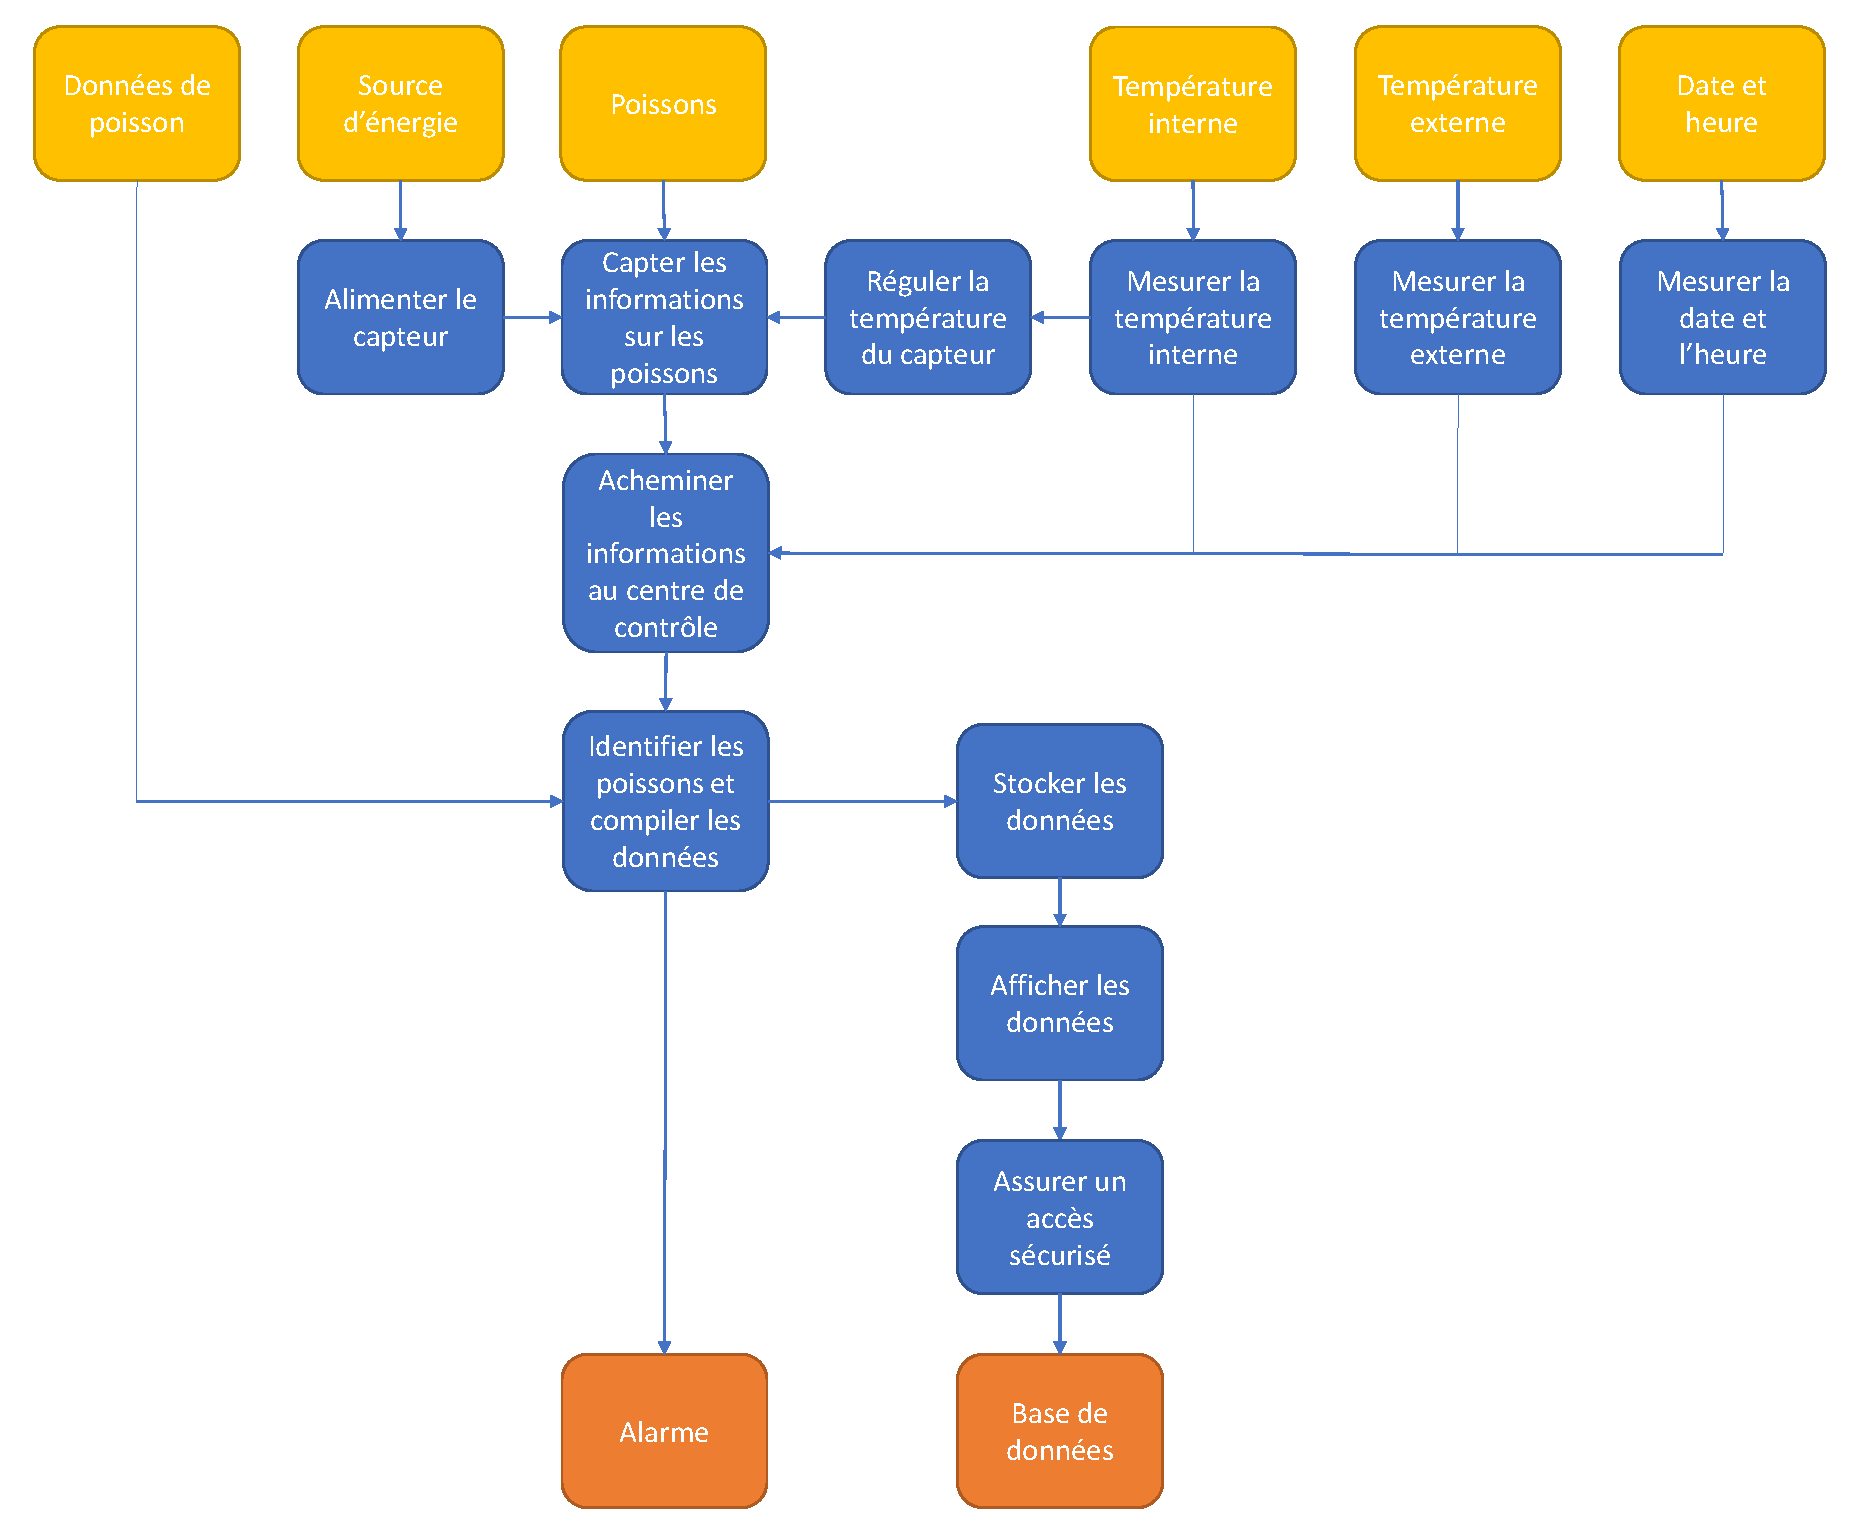
\includegraphics[width=0.85\linewidth]{fig/Diagramme_fonctionnel.pdf}
    \caption{Diagramme fonctionnel du projet Fish \& Chips}
    \label{fig:diagramme_fonctionnel}
\end{figure}

La figure \ref{fig:diagramme_fonctionnel} présente le diagramme fonctionnel du design pour le projet Fish \& Chips. Les intrants y sont présentés en jaune, les fonctions en bleu et les extrants en rouge.

Les intrants constituent toutes les données nécessaires au projet que l'on extrait de l'environnement. Les poissons sont au coeur du projet: à l'aide d'une mesure passive, ils devront être analysés et identifiés par un système de reconnaissance. Le MFA souhaite comptabiliser les espèces de poissons d'eau douce du Québec qui font plus de 6 cm de long. Pour ce faire, des données de poissons seront fournies au système de reconnaissance. Elles seront sous une forme de base de données qui comprendra plusieurs photos de poissons de chaque espèce sous différents angles de vue avec leur espèce correspondante. Ensuite, une source d'énergie sera tirée de l'environnement ou d'une composante pour alimenter le dispositif qui sera chargé de capter les données brutes sur les poissons. La température interne du dispositif de mesure des poissons, la température de l'eau ainsi que la date et l'heure sont nécessaires à la création de la vignette. De plus, certaines de ces données serviront à déterminer s'il y a une erreur dans le système pour avertir un utilisateur.

Les extrants sont les produits du système. Le point central du design est de produire une base de données contenant toutes les vignettes de poissons identifiés, les statistiques sur les populations des différentes espèces, les images originales enregistrées pour une durée de 2 ans ainsi que d'autres informations connexes comme les commentaires, les paramètres de configuration et les alarmes. Les alarmes seront envoyées à un responsable sous la forme d'un message lui avertissant que le fonctionnement du système peut être compromis.

%\pagebreak

\section{Conceptualisation et analyse des solutions}

\subsection{Capter les informations sur les poissons}

Afin d'optimiser et de faciliter l'identification des poissons, il est nécessaire d'utiliser un système de détection de qualité. En ce sens, il est primordial que le capteur optique utilisé soit fiable et efficace. Le capteur optique a comme responsabilité de détecter les poissons de même que prendre une image de ceux-ci. Cependant, son utilisation ne doit en aucun cas perturber l'environnement de la faune aquatique.


\textbf{Aspects physiques:}
\begin{itemize}[label = {--}]
    \item Sous l'eau, la solution accompagnée des autres concepts doit posséder une masse inférieure à 5kg.
    \item Sous l'eau, la solution accompagnée des autres concepts doit posséder un volume de moins de 0.3m$^3$.
    \item L'ensemble du système doit être utilisable jusqu'à une profondeur de 50 pieds.
    \item La température interne de la solution doit rester entre -6°C et 30°C.
\end{itemize}

\textbf{Aspects économiques:}
\begin{itemize}[label = {--}]
    \item La solution doit être la moins dispendieuse possible.
\end{itemize}

\textbf{Aspects temporels:}
\begin{itemize}[label = {--}]
    \item Le temps de développement de la solution doit être minimisé.
    \item Le temps de livraison de la solution doit être minimisé.
\end{itemize}

\textbf{Aspects socio-environnementaux:}
\begin{itemize}[label = {--}]
    \item La solution doit assurer une mesure passive.
\end{itemize}

\subsubsection{GoPro Hero7 Black Edition}

\textbf{Description:} La GoPro Hero7 Black comporte plusieurs fonctionnalités. Elle peut prendre des images de 12 méga-pixels. Elle comprend un système de stabilisation d'images idéal pour la détection de poissons et un mode pour la vision nocturne. Sa fonctionnalité « Live Streaming » ainsi que son système de connexion Wi-Fi et Bluetooth intégré permettraient également de relever les données sur les poissons en temps réels. Un système intégré GPS permet de la localisé en tout temps. La GoPro coûte 560\$. Pour la luminosité, on utilisera une petite lumière DEL Everlight 334-15/T2C1-1WYA blanche compatible avec un Rasberry Pi au coût de 2\$.

\textbf{Décision:} Retenu, mais.

\textbf{Justification:} La GoPro Hero7 Black Edition comporte de nombreux avantages et réponds aux exigences du client. En effet, la masse de la caméra est de 0,116kg et son volume est de 9,2309x10$^{-5}$m$^3$. Il s'agit d'une caméra très fiable et utilisée dans des conditions climatiques extrêmes. Cependant, la GoPro peut seulement atteindre une profondeur de 33 pieds. Des frais additionnels d'environ 67\$ sont donc nécessaire pour l'achat d'un boîtier de plongée permettant à la caméra d'atteindre une profondeur de 196 pieds.

\textbf{Références:} \cite{GoPro_Specs} \cite{GoPro_Waterproof} \cite{DEL}


\subsubsection{HP2W Hyperfire 2 Professionnal White Flash Camera}
\label{subsubsectionHyperfire}

\textbf{Description:} Conçu pour la chasse, cette caméra offre beaucoup de fonctionnalités intéressantes dans le cadre du projet Fish \& Chips. La HP2W peut prendre des images de 3 méga-pixels et des vidéos de 720p à haute définition. La caméra peut ainsi prendre entre 5 et 450 images par secondes. Elle peut fonctionner à des températures allant de -40°F à +140°F et elle possède un détecteur de mouvements et un flash intégré pour la nuit. Son prix incluant les frais de livraison monte à environ 660\$.

\textbf{Décision:} Retenu, mais.

\textbf{Justification:} Cette caméra de chasse professionnelle répond à l'ensemble des exigences du projet. Elle possède une masse de 0,380kg et un volume de 1,0143x10$^{-3}$m$^3$. La HP2W respecte également les contraintes de températures. Aucune informations concernant l'étanchéité du produit est spécifié. Le boîtier est néanmoins capable de résister à des fortes tempêtes de pluie.

\textbf{Références:} \cite{HP2W}


\subsubsection{GoFishCam}

\textbf{Description:} La GoFishCam est une caméra utilisée pour la pêche. Elle peut enregistrer des vidéos de 1080p. La résolution peut ainsi atteindre environ 2 Mégapixels. Elle peut prendre entre 30 et 60 images par seconde. Cette caméra est conçue avec du matériel militaire et sa forme aérodynamique permet une stabilisation d'image lors de l'enregistrement. La GoFishCam comprend des diodes électroluminescentes (LEDs) efficace pour la vision de nuit. Son prix s'élève à environ 325\$ et est livrable entre 10 et 15 jours.

\textbf{Décision:} Retenu.

\textbf{Justification:} La GoFishCam comprend étonnamment des spécifications techniques adéquates pour le projet. En effet, la caméra peut atteindre une profondeur de près de 500 pieds et possède une masse de 0,094kg. La GoFishCam respecte également les contraintes reliées au volume. En effet, elle possède un volume d'environ 8,624x10$^{-5}$m$^3$. La caméra possède également un système de Wi-Fi intégré et une fonction « Live Stream » permettant la diffusion en directe sur une application.

\textbf{Références:} \cite{GoFishCam} \cite{GoFishCam_resolution}


\subsubsection{Capteur d'image OV5640}
\label{subsubsection:camera_custom}

\textbf{Description:} Cette solution permet de créer notre propre caméra à l'aide du capteur d'image CMOS OV5640 (modèle ELP-USB500W02M-AF60). Ce capteur permet d'enregistrer des images de 5 méga-pixel. Le capteur peut prendre des images des objets situés entre 5cm et 100m de la lentille. Ce capteur peut être opérationnel à des températures variant entre -20°C et 70°C. Il s'agit d'un système complètement programmable par port USB. Par ailleurs, puisque le capteur ne peut être submergé, il aurait un boîtier fait en aluminium 2014-T6 et une fenêtre en PMMA (comme montré à la figure \ref{fig:boitier_camera_custom}). Il serait contenu dans un volume de 0.04m$^3$ et il aurait une masse totale de 2.25kg avec les données de l'annexe \ref{annexe:equation_boitier}.

\textbf{Décision:} Retenu, mais.

\textbf{Justification:} Le principal avantage de la création d'un système de capture d'image est le coût. En effet, un tel système coûte seulement 60\$ et est livrable entre 3 et 13 jours. Les coûts du boîtier sont présentés à la table \ref{t:commande_boitier}. Il respecte aussi les contraintes de température. Une telle conception respecte également les spécification requise à la qualité d'image. Cependant, un tel système est davantage complexe puisqu'il faut s'assurer de l'étanchéité du capteur. Pour ce faire, il est possible de souder 6 plaques d'aluminium ensemble dont l'une ayant un vitre en PMMA encastrée. Dans le cadre du projet, la pression à 15.25m est de 251kPa. L'aluminium résiste jusqu'à une pression de 414MPa et le PMMA résiste jusqu'à une pression de 45MPa, ce qui est amplement suffisant pour le projet Fish \& Chips.

\textbf{Références:} \cite{OV5640} \cite{OV5640_coûts} \cite{ASM} \cite{Glass}

\begin{table}[!htb]
\footnotesize
\centering
\scalebox{1.1}{
    \begin{tabular}{|c|c|c|c|c|c|}
    \hline
    \multirow{2}{*}{Concepts} & \multicolumn{4}{c|}{Aspects de l'analyse} & \multirow{2}{*}{Décision} \\ \cline{2-5}
    & Physiques & Économiques & Temporels & Socio-envir & \\
    \hline\hline
    GoPro Hero7 Black & Oui, mais & Oui & Oui & Oui & Retenu, mais\\
    HP2W Hyperfire 2 & Oui, mais & Oui & Oui & Oui & Retenu, mais \\
    GoFishCam & Oui & Oui & Oui & Oui & Retenu \\
    Capteur OV5640 & Oui, mais & Oui & Oui & Oui & Retenu, mais \\
    \hline
    \end{tabular}
}
\caption{Faisabilité des concepts pour capter les informations sur les poissons}
\label{t:Decision_capteur}
\end{table}

\subsection{Alimenter le capteur}
 Cette fonction permet l'alimentation en énergie du système. C'est une fonction assez importante car le système a besoin d'énergie pour fonctionner. Le client demande un système capable de fonctionner 24 heures sur 24 pour une durée minimum de 14 jours en zone éloignée. Ainsi les aspects que nous utiliserons pour évaluer les critères de faisabilités sont les suivants : 
 \textbf{Aspects physiques:}
 \begin{itemize} [label = {--}]
    \item Dimensions de la solution, intensités et fiabilité de la solution. La solution doit opérer pendant au moins 14 jours ou encore 50mAh.
\end{itemize}
 \textbf{Aspects économiques:}
 \begin{itemize} [label = {--}]
    \item La solution doit être la moins coûteuse possible.
\end{itemize}
 \textbf{Aspects temporels:}
 \begin{itemize} [label = {--}]
    \item Disponibilité de la solution.
\end{itemize}
 \textbf{Aspects socio-environnementaux:}
 \begin{itemize} [label = {--}]
    \item Le système doit être sécuritaire pour l'environnement.
\end{itemize}
\subsubsection{Batterie au lithium :}

\textbf{Description :}
Pour alimenter notre système, on peut se servir des batteries au lithium telle que Energizer Ultimate Lithium. Ces piles, lorsqu'elles sont utilisées dans certains capteurs comme la caméra HP2W Hyperfire 2 (voir \ref{subsubsectionHyperfire}), ont une durée de vie s'étalant sur deux ans ou encore 40000 images ce qui nous permettra de répondre aux attentes du client. En plus d'une bonne durée de vie, les coûts de ces batteries sont très bas, on parle de 17.87\$ la douzaine chez Walmart. Elles sont également performantes dans les températures extrêmes allant de -40°C à 60°C. Ces batteries de 1.5V ne sont pas rechargeables et ne présentent pas de risques pour l'environnement.
 
 \textbf{Décision :}
 Retenu.
 
 \textbf{Justification :}
 Peu coûteuse et facilement accessible chez plusieurs fournisseurs, cette option respecte nos contraintes économiques et temporels. Aussi en empilant un certain nombre de ces batteries on aboutie à une alimentation fiable et sécuritaire. De cette manière, nos contraintes physiques et socio-environnementaux sont également respectées.
 
\textbf{Références:} \cite{Lithium}

\subsubsection{Batterie Power Bank :}
\textbf{Description :}
 Ce concept consiste à se servir de Power Bank de type Anker qui n'est rien d'autre qu'un chargeur portable pour alimenter notre système. Il a une haute puissance avec sortie de 4.8A . Le voltage de sortie est de 5V. Ce type de chargeur est disponible pour livraison chez Best Buy dans les 5 jours ouvrables suivant la date de l'achat, et ce, au prix de 69.09\$. Les dimensions sont approximativement de 14.5 cm pour la longueur, 6 cm pour la largeur et 2.5 cm pour la hauteur. Il faut noter que la batterie doit être fixée dans la boite contenant le système et relié à ce dernier par un câble.
 
\textbf{Décision :}
 Rejeté.
 
\textbf{Justification :}
Avec cette option on pourra certes répondre à la demande du client mais il faudra associer, c'est à dire, mettre en série au moins trois batteries. Ce qui fera augmenter la facture et aussi utilisera beaucoup trop d'espace  dans la boite du système.
 
\textbf{Références:} \cite{Power_Bank}
 
\subsubsection{Alimentation Filaire:}
\textbf{Description :}
Pour le 3e concept, il s'agit de l'alimentation filaire. Pour cette solution, le système sera directement relié a une prise électrique située à la surface par l'entremise d'un câble d'alimentation. Si nécessaire, plusieurs cordons seront enfilés pour avoir une longueur maximale. On utilisera la rallonge filaire de 50 pieds pour 39,00\$ sur uline.ca.
 
 \textbf{Décision :}
 Retenu.
 
 \textbf{Justification :}
 La solution filaire, en plus de réduire les coûts, permet d'alimenter constamment le système dans une configuration sécuritaire.
 
 \textbf{Références :} \cite{fil}
 
\subsubsection{Panneaux solaires:}

\textbf{Description :}
Le panneau solaire externe donne également une autre possibilité pour alimenter notre système. Il est muni d'un coffre de 8x8 pouces qui contient une batterie rechargeable de 12V avec prise d'alimentation externe, qui est rechargée en permanence par le panneau solaire via un câble de 3 pouces. Avec une puissance de 7 watts et des dimensions de 13x14 pouces, le panneau solaire est une option un peu plus dispendieuse. Son prix est de 299.99\$ livrable dans les 5 jours ouvrables suivant la date de l'achat. Ce prix inclut tout le câblage ainsi que le matériel de montage. Le principal avantages de cette option est la permanence de l'énergie qui permettra à notre système de fonctionner sans interruption.

\textbf{Décision :}
Retenu, mais.

\textbf{Justification :}
Le concept du panneau solaire respecte nos contraintes, mais il faut mentionner qu'il peut constituer un danger lorsqu'il est mal installé.


\textbf{Références:} \cite{Panneau_solaire}

\begin{table}[!htb]
\footnotesize
\centering
\scalebox{1.1}{
    \begin{tabular}{|c|c|c|c|c|c|}
    \hline
    \multirow{2}{*}{Concepts} & \multicolumn{4}{c|}{Aspects de l'analyse} & \multirow{2}{*}{Décision} \\ \cline{2-5}
    & Physiques & Économiques & Temporels & Socio-envir & \\
    \hline\hline
    Batterie au lithium & Oui & Oui & Oui & Oui & Retenu\\
    Batterie Power Bank & Non & Oui, mais & Oui & Oui & Rejeté \\
    Filaire & Oui & Oui & Oui & Oui & Retenu \\
    Panneaux solaires & Oui & Oui, mais & Oui & Oui, mais & Retenu, mais  \\
    \hline
    \end{tabular}
}
\caption{Faisabilité des concepts pour l'alimentation du système}
\label{t:Decision_alimenter}
\end{table}

\subsection{Acheminer les informations au centre de contrôle}
Cette composante se devra de transférer les données brutes de poissons, de température et de l'heure à un poste de contrôle pour les traiter et les compiler. Elle agit donc en tant que connexion entre le capteur et le poste de contrôle. Il est à considérer que le capteur peut se situer jusqu'à 15.25m sous l'eau et que les informations doivent être acheminées à une distance d'au moins 50m à travers l'eau comme montré à la figure \ref{fig:distance_acheminer}.

 \textbf{Aspects physiques:}
 \begin{itemize} [label = {--}]
    \item Doit pouvoir acheminer les données au travers de l'eau jusqu'à une distance de 50m.
    \item Doit résister aux différentes conditions environnementales comme les conditions météorologiques et la faune et la flore aquatique.
\end{itemize}

 \textbf{Aspects économiques:}
 \begin{itemize} [label = {--}]
    \item Doit être le moins coûteux possible.
\end{itemize}

 \textbf{Aspects temporels:}
 \begin{itemize} [label = {--}]
    \item N/A.
\end{itemize}

 \textbf{Aspects socio-environnementaux:}
 \begin{itemize} [label = {--}]
    \item Ne doit pas être polluant pour la faune et la flore.
\end{itemize}

\subsubsection{Utilisation de la connexion intégrée au capteur}
\textbf{Description :} La GoPro Hero7 Black et la GoFishCam ont déjà une connexion WiFi intégrée. Il serait possible d'utiliser ces connexions pour communiquer avec le poste de contrôle via un téléphone intelligent. Le choix se pose sur le iPhone 7. Pour les deux capteurs, la connexion Wifi serait à une fréquence de 2.4GHz avec un débit de 78 Mbps. La portée serait de 50 pieds. Le coût de cette solution sera déterminé par le coût du téléphone intelligent, soit 629 \$. À chaque deux semaines, un opérateur pourrait recueillir les données enregistrées sur le iPhone et les envoyer dans le logiciel pour le traitement.

\textbf{Décision :} Retenu, mais.
 
\textbf{Justification :} Dans les deux cas, le transfert de données se fait via une application de téléphone intelligent. Comme le WiFi intégré dans les capteurs ne sont pas optimisés en distance, il faut que le téléphone soit submergé et alimenté en tout temps pour recueillir les données. Considérant que la batterie d'un iPhone est de 1400mAh et qu'il faut l'alimenter durant au minimum 14 jours, cela augmente drastiquement la consommation d'électricité du système. De plus, pour garder le iPhone submergé, le système devra inclure un boîtier. Le système se complexifie grandement pour une fonction qui est relativement simple. En ajoutant un boîtier à 20\$, le coût de cette composante du système s'élève à environ 650\$. Considérant que les coûts en matériel sont limités à 10 000\$, le coût de cette composante est acceptable. De plus, ce concept ne constitue pas un danger de pollution pour les poissons.

\textbf{Références:} \cite{GoPro_Specs} \cite{GoPro_Waterproof} \cite{GoFishCam} \cite{iPhone7}

\subsubsection{Connexion filaire}
\textbf{Description :} Cette solution serait un fil qui relie directement le capteur au poste de contrôle. Ce serait le fil 50m Fibre Optic USB 3.0 Cable de Lindy. Il s'agit d'un fil qui convertit les données numérique en signal optique pour acheminer les données à travers une fibre optique. Le coût de ce file est de 700\$. Une couche protectrice HWN0.13BK - Flexo Heavy Wall 3.18mm en PET sera ajoutée pour assurer la résistance du dispositif. Son coût pour une distance de 250ft (76.2m) est de 82.50\$. Le coût total est donc de 782.50\$.
 
\textbf{Décision :} Retenu.
 
\textbf{Justification :} Avec la couche protectrice, le fil à fibre optique pourra résister à l'eau et à certains chocs malgré la fragilité de la fibre optique. En effet, la gaine protectrice est prévue pour des applications marines et industrielles et peut résister au contact constant avec des surfaces abrasives, comme la terre et la roche. Avec une atténuation nominale de 2.5dBm/km, le signal optique parcourra avec les 50m avec très peu de pertes. Le fil de fibre optique peut opérer entre 0°C et 50°C, ce qui couvre l'intervalle de température de l'eau (4 à 25°C). Il remplit donc facilement les contraintes physiques reliées au projet. Comme mentionné précédemment, avec un budget en matériel de 10 000\$, il est sécuritaire de dire que ce concept remplit aussi les contraintes économiques. Le fil ne cause pas de pollution dans l'eau.

\textbf{Références:} \cite{usb_50m} \cite{usb_standard_50m} \cite{Techflex}

\subsubsection{Utilisation d'un Raspberry Pi}
\textbf{Description :} Le Raspberry Pi peut accueillir jusqu'à 4 périphériques USB ainsi qu'une connexion WiFi. En installant un routeur au poste de contrôle et en reliant le capteur au Raspberry Pi, il serait possible de communiquer par WiFi. Une connexion standard 802.11N serait utilisée à 2.4GHz et un débit maximal de 750 Mbps. La portée d'une telle connexion peut aller jusqu'à 250m. Le coût d'un Raspberry Pi 3 – Modèle B Plus est de 46.50\$. Le routeur Synology RT2600ac à 250\$ peut accueillir le standard WiFi souhaité.

\textbf{Décision :} Retenu, mais.
 
\textbf{Justification :} Les ondes électromagnétiques dans les RF sont atténuées par les propriétés conductrices de l'eau ce qui pourrait compromettre l'acheminement de l'information. Cependant, comme la conductivité de l'eau douce est faible, il est possible de propager des signaux à 2.4GHz sans trop de pertes. Il faut tout de même savoir que la signal WiFi se propage en ligne droite et que la majorité de son trajet sera sous l'eau. Un tel système de pourra donc pas être trop loin du poste de contrôle. Les contraintes physiques sont donc remplies, mais ce concept comporte certaines limites. Le coût est raisonnable et les ondes EM n'interfèrent pas avec la faune et la flore aquatique. Les deux autres contraintes sont donc remplies. 

\textbf{Références :} \cite{Raspberry_Pi} \cite{Routeur} \cite{eau_EM}

\subsubsection{Acheminement manuel}
\textbf{Description :} Plusieurs capteurs comportent déjà une mémoire interne sous forme de carte SD et il serait intéressant d'en tirer profit. Puisque le système doit être complètement autonome pour une durée d'au moins 14 jours, un opérateur pourrait venir récolter les informations sur la mémoire interne des capteurs à chaque deux semaines. Les données seraient ensuite transférées au poste de contrôle pour le traitement.
 
\textbf{Décision :} Retenu.
 
\textbf{Justification :} Les mémoires internes des cartes SD peut aller jusqu'à 512Go, ce qui couvre largement la tailles des données enregistrées pendant 2 semaines. La durée du transfert de données serait donc de deux semaines, mais comme, il n'est pas nécessaire d'avoir accès aux données en temps réel, c'est un délai qui reste raisonnable pour la création d'une base de données. De plus, il ne s'agit pas d'une grande corvée puisqu'il y a de grandes chances que l'opérateur doive recharger le capteur de toute façon. Si le capteur est muni d'une carte SD, le coût est nul et sinon, il serait d'une quarantaine de dollars. Il s'agit d'une solution qui remplit les trois critères demandés.

\begin{table}[!htb]
\footnotesize
\centering
\scalebox{1.0}{
    \begin{tabular}{|c|c|c|c|c|c|}
    \hline
    \multirow{2}{*}{Concepts} & \multicolumn{4}{c|}{Aspects de l'analyse} & \multirow{2}{*}{Décision} \\ \cline{2-5}
    & Physiques & Économiques & Temporels & Socio-envir & \\
    \hline\hline
    Connexion intégrée au capteur & Oui, mais & Oui & N/A & Oui & Retenu, mais\\
    Connexion filaire & Oui & Oui & N/A & Oui & Retenu \\
    Raspberry Pi & Oui, mais & Oui & N/A & Oui & Retenu, mais \\
    Manuel & Oui & Oui & N/A & Oui & Retenu \\
    \hline
    \end{tabular}
}
\caption{Faisabilité des concepts pour l'acheminer des données brutes}
\label{t:Decision_acheminer}
\end{table}
 

\subsection{Identifier les poissons}

Cette composante a pour fonction de transformer et compiler les données brutes recueillies par les différents capteurs pour créer les vignettes. Elle devra donc être en mesure d'identifier les espèces de poissons à partir des données du capteur. De plus, elle se chargera de comptabiliser le nombre de poissons de chaque d'espèces et de produire des statistiques. Cette fonction traitera aussi si une alarme doit être générée. Il y aura une alarme lorsque le fonctionnement du système pourrait être compromis, c'est-à-dire si il y la température interne excède l'intervalle de résistance à la température des composantes du capteur, si l'identification est impossible sur plusieurs captures ou si il y a une brèche de sécurité.

L’automatisation de la prise de données sur les poissons étant au cœur du projet de conception, il est important de considérer l’ensemble des opportunités qui se présentent avec un budget de développement de 40 000\$. Le projet devant être profitable à long terme, la considération du coût et du temps de développement seront pris en compte, mais également la facilité de configuration pour le déploiement dans différents sites. Le facteur du 5 poissons à détecter par site peut également jouer en ligne de compte sur la complexité de l’algorithme à développer, c’est pourquoi il sera pris en compte. Le logiciel doit être fiable, opérationnel en tout temps et ne comporter aucun bug. Une solution présentée pourrait demander du matériel pour une collecte de données au préalable avant le déploiement du système, c’est pourquoi ce critère sera abordé seulement dans cette section. 


 \textbf{Aspects physiques:}
 \begin{itemize} [label = {--}]
    \item La collecte de donnée (si applicable) devra utiliser le moins de matériel possible et détecter les poissons avec justesse.
\end{itemize}

 \textbf{Aspects économiques:}
 \begin{itemize} [label = {--}]
    \item Les coûts de développement du système se doivent d’être minimisés le plus possible, sans dépasser la limite de 40 000\$.
\end{itemize}

 \textbf{Aspects temporels:}
 \begin{itemize} [label = {--}]
    \item Le temps de développement de la solution doit être minimisé.
\end{itemize}

 \textbf{Aspects socio-environnementaux:}
 \begin{itemize} [label = {--}]
    \item N/A.
\end{itemize}

\subsubsection{Réseau de neurones convolutionnel avec la librairie Tensorflow :}

\textbf{Description :} Pour l’analyse visuelle et la reconnaissance intelligente de types de poissons, l’apprentissage profond de type convolutionnel conviendrait bien aux besoins du client. Le principe d’une telle méthode d’apprentissage ressemble drôlement au processus d’apprentissage animal : on entre des milliers de photos en entrée et on évalue ensuite la sortie de l’ordinateur lorsque le logiciel exécute une reconnaissance. On répète les opérations jusqu’à temps que le logiciel aille un fort taux de précision. Il est difficile de mettre un nombre exact sur le temps de développement et le nombre de photos en entrées pour l’apprentissage du logiciel. Par contre, plus le temps de développement et le nombre de photos en entrée sont élevées, plus la précision de détection du logiciel augmentera.  Pour mettre le tout simplement, le capteur sera composé d’un programme déclenchant la prise de photo suite à un entraînement, et la création de la vignette s’opérera au centre de contrôle placé à l’extérieur de l’eau. Le désavantage ici est évidemment la quantité de photos utilisées et le temps nécessaire pour le développement du programme, car une bonne précision demandera une durée et un nombre de photos importants. De plus, un changement de site impliquerait un réapprentissage partiel du programme, ce qui signifierait potentiellement une augmentation des coûts de développement à long terme.

\textbf{Décision :} Retenu.

\textbf{Justification :} L’utilisation de la technologie d’apprentissage machine répondrait parfaitement aux besoins du client et serait autonome dans sa prise de mesure. Le processus d’apprentissage s’avère long et demande un bon nombre de ressources en images, mais à long terme, le logiciel peut s’avérer plus profitable, plus exact et plus précis que la majorité des autres options présentées plus bas. 

\textbf{Références :} \cite{tensorflow}


\subsubsection{Logiciel simple de création de masque et de détection de forme :}

\textbf{Description :} Un algorithme moins coûteux que celui présenté plus haut consiste en un traitement d’image par création de masques. Le principe est la création de photos noirs et blancs selon la détection de formes, de contours et de changements de couleurs (« edge detection »). Il serait ensuite possible de superposer les masques des poissons capturés par la caméra avec ceux d’une librairie préinstallée sur le système et calculer l’intersection du nombre de pixels blancs correspondants. Il est à noter que l’ajout d’un flou gaussien devrait améliorer la détection des formes et des couleurs. Avec un taux de ressemblance allant dans les hauts pourcentages (90\% à 100\%), on dira que le poisson sera identifié avec justesse. La seule limitation de cette technique se présentera lors de la création de la librairie : la qualité de la reconnaissance dépendra grandement de la qualité des photos utilisées. On devra donc utiliser une grande base de données de poissons, telle que FishBase, ou bien capturer le poisson de chaque espèce à détecter et prendre des photos dans tous les angles pour s’assurer d’une bonne détection du logiciel. 

\textbf{Décision :} Rejeté.

\textbf{Justification :} Cette option est avantageuse en raison du faible nombre de poissons à détecter, ce qui ne nécessiterait pas nécessairement un logiciel d’apprentissage profond. Par contre, on aura tendance à prioriser un logiciel plus efficace et fiable dans sa prise de mesure pour un projet de calibre professionnel. À long terme, on aura avantage à investir dans une détection de poisson plus fiable qu’une simple superposition de masques.

\textbf{Références :} \cite{requinage}


\subsubsection{Développement par un Tiers}

\textbf{Description: }L’établissement d’un partenariat avec une compagnie établie en intelligence artificielle pourrait également être envisageable dans la conception du logiciel de détection de poissons. Toute compagnie établie dans le domaine de l’intelligence artificielle, telle que la compagnie Element AI à Montréal, et qui possède de l’expertise en vision numérique pourrait amener de son expertise au projet et développer un logiciel de reconnaissance d’espèces de poisson avec aise. Le coût de développement d’un tel logiciel peut s’avérer coûteux. Puisqu’il est difficile de mettre un chiffre exact sur les tarifs d’une compagnie en particulier, on estimera les coûts de développement à  35 000\$.

\textbf{Décision :} Retenu.

\textbf{Justification :} le développement d’un logiciel par une compagnie experte dans l’intelligence génèrerait nécessairement un logiciel de grande qualité. Le seul désavantage dans une telle solution serait le coût de production. D’un autre côté, on peut s’assurer d’une qualité de production supérieure, donc profitable à long terme.

\textbf{Référence :} \cite{elementai}


\subsubsection{FishVerify App}

\textbf{Description :} Il existe aussi déjà des solutions logicielles potables sur le marché donnant des approximations sur l’espèce d’un poisson : il est ainsi possible de réduire les coûts de production en amorçant le développement du logiciel à partir d’une application déjà fonctionnelle. Il serait possible tout en l’adaptant à notre situation. Un partenariat avec une compagnie telle que FishVerify, une application de détection de poisson pour la pêche, pourrait être un excellent point de départ dans la création d’un logiciel tel que demandé par le ministère. L’avantage de cette solution est la réduction des coûts, mais également la réduction de temps nécessaire pour développer le produit.

\textbf{Décision :} Rejeté.

\textbf{Justification :} On peut s’assurer d’un produit fonctionnel et efficace avec une telle optique de production. Puisqu’on amorce le projet avec un produit fonctionnel, on peut s’assurer d’un produit fonctionnel et adapté aux besoins du ministère en peu de temps. Bien que la solution soit intéressante, le produit possède une banque de données inapproprié pour le territoire du Québec. En effet, la banque de données de FishVerifyApp comprend environ 150 poissons communs de la Floride. De plus, il faut souligner que la contrainte du partenariat peut facilement rendre cette solution inconvéniente.


\textbf{Références :} \cite{fishverify}


\begin{table}[!htb]
\footnotesize
\centering
\scalebox{1.0}{
    \begin{tabular}{|c|c|c|c|c|c|}
    \hline
    \multirow{2}{*}{Concepts} & \multicolumn{4}{c|}{Aspects de l'analyse} & \multirow{2}{*}{Décision} \\ \cline{2-5}
    & Physiques & Économiques & Temporels & Socio-envir & \\
    \hline\hline
    Réseau de neurones & Oui  & Oui & Oui & Oui & Retenu \\
    Logicel par détection de masque & Non & Oui & Oui & Oui & Rejeté \\
    Développement par un tiers & Oui & Oui, mais & Oui & Oui & Retenu \\
    FishVerify app & Non & Oui, mais & Oui & Oui & Rejeté \\
    \hline
    \end{tabular}
}
\caption{Faisabilité des concepts pour identifier les poissons et compiler les données}
\label{t:Decision_identifier}
\end{table}


\subsection{Compiler les données}
Ce dispositif a pour fonction d'accueillir le logiciel de reconnaissance et la base de données. Il devra donc avoir une puissance de calcul considérablement élevée puisque l'entraînement d'un logiciel de reconnaissance nécessite une quantité énorme de calculs à effectuer. De plus, c'est à partir de cet appareil que les données sont transmises sur le serveur. Il est aussi établi qu'une source de tension autre que l'alimentation du capteur est fournie et que ce dispositif se situe en dehors de l'eau.

\textbf{Aspects physiques:}
\begin{itemize}[label = {--}]
    \item La solution doit accueillir le logiciel de reconnaissance et la base de données.
    \item La solution doit entraîner le logiciel de reconnaissance le plus rapidement possible.
\end{itemize}

\textbf{Aspects économiques:}
\begin{itemize}[label = {--}]
    \item La solution doit être la moins dispendieuse possible.
\end{itemize}

\textbf{Aspects temporels:}
\begin{itemize}[label = {--}]
    \item N/A
\end{itemize}

\textbf{Aspects socio-environnementaux:}
\begin{itemize}[label = {--}]
    \item N/A
\end{itemize}

\subsubsection{Raspberry Pi}

\textbf{Description :} Le Rapsberry Pi 3 Modèle B+ est un microprocesseur opérant sur Raspbiant, un système d'exploitation se rapportant à une branche de Linux. Il est muni d'un port WiFi intégré qui suit la norme 802.11.b/g/n/ac à 2.4 et 5GHz de l'IEEE ainsi qu'un microprocesseur ARM Cortex-A53 lui permettant d'atteindre une vitesse de 1.4 GHz. Il a aussi un port GPIO avec 40 tiges. Son coût est de 46.50\$.

\textbf{Décision :} Rejeté.

\textbf{Justification :}  Le port GPIO présente un aspect pratique important: il serait possible de brancher les capteurs de température directement sur le Raspberry Pi si il est submergé avec le capteur. Il faudrait cependant s'assurer que la batterie puisse alimenter le capteur ainsi que le Raspberry Pi. Par contre, ce microprocesseur n'a pas de carte graphique. La puissance de calcul repose donc entièrement sur le processeur et celui-ci n'est pas assez performant pour une telle application. Pour cette raison, le concept est rejeté malgré son coût très peu élevé.

\textbf{Références :} \cite{Raspberry_Pi_Specs}
 
 
\subsubsection{Alienware Aurora R7}

\textbf{Description:} Cet ordinateur propose des composantes coûteuses mais performantes. Il est doté d'un processeur Intel Core i7-8700 à 3.2 GHz, une mémoire vive de 16 Go, un disque dur intégrée de 1 To ainsi qu'une carte graphique NVIDIA GeForce GTX 1060-6Go. Il a aussi un port de connexion WiFi 802.11ac. Il est possible de l'acquérir au prix de 1700\$ chez BestBuy.

\textbf{Décision:} Retenu.

\textbf{Justification:} Le disque dur interne intégré de 1 To peut être avantageux puisqu'il serait possible de l'utiliser afin de stocker les données. De plus, sa carte graphique est très performante ce qui lui permettrait d'effectuer l'entraînement du logiciel de reconnaissance assez rapidement. Sa connexion WiFi lui permettrait aussi de communiquer avec le capteur via un réseau WiFi et ainsi faire le transfert de données lorsque possible. Il rempli donc les critères physiques imposés et propose même un avantage pratique. Finalement, son coût de 1700\$ est raisonnable puisque le budget alloué en matériel est de 10000\$.

\textbf{Références:} \cite{User_Benchmark_score} \cite{Alienware_R7} 


\subsubsection{Hp Pavilion Power 580-130}

\textbf{Description:} Le HP Pavilion Power 580-130 a une mémoire vive de 8 Go, un disque dur interne de 1 To ainsi que la possibilité d'une connexion WiFi. Il a un processeur Ryzen 5 d'AMD qui lui permet d'atteindre une vitesse de 3.2 GHz. Avec une carte graphiqe d'AMD Radeon RX 580, il est possible de l'acheter pour la somme de 950\$ chez Walmart.

\textbf{Décision:} Retenu.

\textbf{Justification:} Malgré des composantes plus modestes, cet ordinateur serait capable d'offrir une bonne puissance calcul à un prix moins élevé. En effet, sa carte graphique fait tout de même partie des meilleures disponibles sur le marché et elle serait amplement suffisante pour la charge computationnelle. Son disque dur interne et sa connexion WiFi procurent eux aussi un avatage pratique poru les besoins du projet. Avec un prix de 950\$, le HP Pavilion remplit tous les critères émis.

\textbf{Références:} \cite{AMD_RX} \cite{HP_hardware}


\subsubsection{Ordinateur personnalisé}

\textbf{Description:} Il est aussi possible de personnaliser l'ordinateur afin de mieux s'adapter aux besoins. L'ordinateur personnalisé choisi a une carte mère Asus Prime Z370-P à 178\$, un processeur Intel Core i5-8400 à 280\$, une carte graphique RTX GeForce 2070 d'Asus à 737\$, un disque dur de 2 To Barracuda de Seagate à 73\$ et une mémoire vive de 16 Go Vengeance LPX de Corsair à 118\$. La carte mère peut recevoir une connexion WiFi par un fil via un routeur. La somme totale de cet ordinateur serait de 1386\$.

\textbf{Décision:} Retenu.

\textbf{Justification:} L'avantage principal de la personnalisation de l'ordinateur est qu'il peut être optimisé selon les besoins du MFA. En effet, puisque la puissance de calcul est surtout dépendante de la carte graphique, il est possible d'acheter des composantes moins dispendieuses pour allouer plus d'argent sur la carte graphique. Avec la carte graphique RTX GeForce 2070 d'Asus, l'ordinateur remplit largement son mandat. De plus, son coût d'environ 1400\$ est acceptable par rapport au budget de 10000\$ alloué en matériel.

\textbf{Références:} \cite{Custom_R7} \cite{Amazon_RTX} \cite{Amazon_i5}

\begin{table}[!htb]
\footnotesize
\centering
\scalebox{1.0}{
    \begin{tabular}{|c|c|c|c|c|c|}
    \hline
    \multirow{2}{*}{Concepts} & \multicolumn{4}{c|}{Aspects de l'analyse} & \multirow{2}{*}{Décision} \\ \cline{2-5}
    & Physiques & Économiques & Temporels & Socio-envir & \\
    \hline\hline
    Raspberry Pi & Non & Oui & N/A & N/A & Rejeté \\
    Alienware Aurora R7 & Oui & Oui & N/A& N/A& Retenu \\
    HP Pavilion Power 580-130 & Oui & Oui & N/A& N/A & Retenu \\
    Ordinateur personnalisé & Oui & Oui & N/A & N/A & Retenu \\
    \hline
    \end{tabular}
}
\caption{Faisabilité des concepts pour la compilation des données}
\label{t:Decision_compilation}
\end{table}


\subsection{Stocker les données}
La composante qui occupera cette fonction devra enregistrer toutes les données pertinentes pour la base de données, c'est-à-dire les vignettes et les commentaires, les statistiques, les paramètres de configuration, les alarmes  qui ont été envoyées, les données de poissons de référence et les images originales prises par le capteur.
Comme mentionné à la section \ref{subsection:capacite_stockage}, ces données totaliseront un minimum de 200Go.

\textbf{Aspects physiques:}
\begin{itemize} [label = {--}]
    \item Le système soit pouvoir stocker au moins 200 Go de données.
\end{itemize}

\textbf{Aspects économiques:}
\begin{itemize} [label = {--}]
    \item La solution doit être la moins coûteuse possible.
\end{itemize}

\textbf{Aspects temporel:}
\begin{itemize} [label = {--}]
    \item La conception de la solution doit respecter des délais raisonnables.
\end{itemize}

\textbf{Aspects socio-environnementaux:}
\begin{itemize} [label = {--}]
    \item Les données stockées doivent être le plus facilement accessibles aux utilisateurs.
\end{itemize}

\subsubsection{Carte mémoire SD SanDisk 32 Go classe 10 :}

\textbf{Description :} La carte mémoire SD SanDisk 32 Go classe 10 est une carte mémoire utilisée pour conserver les photographies en haute résolution sur les appareils photos compacts et de portée moyenne. Il a une capacité de stockage de 32 Go. Il peut stocker des vidéos en haute définition. La carte mémoire possède également une vitesse de transfert de 80 Mbps. Également, il est dit que cette carte est étanche et résistante aux chocs et aux rayons X. Le système possède également une étiquette inscriptible lors de prise de photos et de vidéos. Elle coûte 13.98 dollars sur Amazon.

\textbf{Décision :} Rejeté.

\textbf{Justification :} Cette carte est très intéressante pour ce projet car elle est étanche, donc, résistante à l’eau et aux chocs et il serait également possible de récupérer les données même en cas de bris de la machine. La carte SD est très intéressante aussi pour sa vitesse de transfert. En effet, elle pourrait transférer ses informations à une vitesse très rapide pour la transmission d’une photographie. Enfin, grâce à l’étiquette inscriptible, il sera plus facile de concevoir la vignette. Cependant, on ne peut pas utiliser la carte SD car elle ne possède pas une capacité suffisante.

\textbf{Références :} \cite{casd} \cite{amsd}

\subsubsection{Cloud de hubiC}
\textbf{Description :} La plateforme Cloud de hubiC est un système informatique en nuage disponible sur la plateforme internet de Google. Un système d’informatique en nuage est un concept permettant d’enregistrer des données sur des ordinateurs localisés à distance grâce à une connexion en ligne et de pouvoir utiliser ces mêmes données à distance des ordinateurs. HubiC est une compagnie qui propose un service de stockage de données par nuage gratuitement jusqu’à 25 Go. Deux autres forfaits sont offert : 15\$ par an pour 100 Go et 75\$ par an pour 10 To. Pour assurer le transfert de données vers les serveurs de hubiC une connexion Internet est nécessaire puis il sera possible de suivre l’évolution des données à partir d’une grande diversité d’appareils (tablette, ordinateurs, téléphones intelligents…). 

\textbf{Décision :} Retenu.

\textbf{Justification :} Grâce à ce système nous pourrions facilement utiliser les données à partir d’un ordinateur. En effet, les données seront directement transmises par Internet, les photographies seraient transférées jusqu’à un ordinateur qui traitera alors les images. On choisit hubiC car il s’agit du système qui garantit gratuitement la plus grande capacité de données en nuage. En acheminant l’information jusqu’au serveur, on pourra alors traiter les informations très rapidement. Pour 75\$ par an, on pourrait parfaitement sauvegarder toutes les données pendant 2 ans et on pourrait y accéder avec n’importe quel ordinateur.

\textbf{Références :} \cite{hubic} \cite{clgo} \cite{incl}

\subsubsection{Disque dur sur SSD Kingston Digital SSD A400 SATA 3 }
\textbf{Description :} Un disque dur sur SSD (Solid State Drive) est un type de disque dur utilisant une mémoire électronique (en opposition aux disque dur mécaniques). Les disques durs représentent un intérêt pour plusieurs raisons : ils sont plus rapides, ils sont silencieux, ils consomment moins d’énergie et ils sont plus résistants aux chocs. Ainsi, cela permet de sauvegarder une quantité importante de données tout en étant très discret et autonome. Cependant, comme c’est un outil de sauvegarde de données fait à base d’électronique, on remarque une usure progressive du système. Le disque dur SSD Kingston Digital SSD A400 SATA 3 proposé par Kingston nous propose 240 Go de données disponible pour 40\$ sur Amazon. 

\textbf{Décision :} Retenu.

\textbf{Justification :} Le disque dur SSD Kingston Digital SSD A400 SATA 3 est un outil pratique pour sauvegarder beaucoup de données. En effet, 240 Go représentent une quantité de données disponible amplement suffisante pour le stockage des données sur la durée établie par le client. Le prix entre également amplement dans les frais matériel établie par le client. Malgré tout, même si l’usure affecte normalement les disques durs, ici, un seul client présente un mécontentement sérieux et ne concerne pas la durée de vie du disque dur.

\textbf{Références :} \cite{AMSSD} \cite{DESSD}

\subsubsection{Disque dur sur HDD Western Digital SATA III }

\textbf{Description :} Les disques durs HDD (Hard Disk Drive) sont des disques durs mécaniques servant à la sauvegarde des données. Ce sont des disques durs mécaniques où l’information est gravée sur des disques tournant à une grande vitesse. Ainsi, on peut accéder aux données gravées même après la fermeture de l’ordinateur qui traite les données. On remarque que les HDD sont moins coûteux que les SSD dans le ratio : données par dollars. Cependant, les HDD sont plus lents que les SSD. Celui proposé par Western Digital permet de stocker 1 To de données pour 54.99\$ sur Amazon. Il a une capacité de 200 000 photographies numériques et il a une garantie de deux ans. 

\textbf{Décision :} Retenu.

\textbf{Justification :} Ce disque dur a une capacité capable de stocker les informations que nous sauvegarderons sur la durée des deux ans. En effet, il peut sauvegarder jusqu’à 1 To. Également, même si elle est moins résistante, en théorie, que le disque dur SSD, il y a une garantie égale à la durée d’utilisation, voulue par le client, de la machine.

\textbf{Références :} \cite{HDD1} \cite{HDD2}

\begin{table}[!htb]
\footnotesize
\centering
\scalebox{0.90}{
    \begin{tabular}{|c|c|c|c|c|c|}
    \hline
    \multirow{2}{*}{Concepts} & \multicolumn{4}{c|}{Aspects de l'analyse} & \multirow{2}{*}{Décision} \\ \cline{2-5}
    & Physiques & Économiques & Temporels & Socio-envir & \\
    \hline\hline
    Carte SD & Non & Oui & Oui & Oui & Rejeté \\
    Cloud & Oui & Oui & Oui & Oui & Retenu \\
    Disque dur SSD & Oui & Oui & Oui & Oui & Retenu \\
    Disque Dur HDD & Oui & Oui & Oui & Oui & Retenu \\
    \hline
    \end{tabular}
}
\caption{Faisabilité des concepts pour le stockage de données}
\label{t:Decision_stockage}
\end{table}



\subsection{Afficher les données}
Cette composante devra afficher les données d'une manière efficace et conviviale pour les employés du MFA. Cette interface assurera la communication avec l'utilisateur pour visualiser les données et configurer les différents paramètres de la caméra comme le focus, l'ISO et la durée d'exposition. \

\textbf{Aspects physiques:}
\begin{itemize} [label = {--}]
    \item N/A
\end{itemize}

\textbf{Aspects économiques:}
\begin{itemize} [label = {--}]
    \item La solution doit satisfaire un excellent rapport qualité/prix.
\end{itemize}

\textbf{Aspects temporel:}
\begin{itemize} [label = {--}]
    \item La conception de la solution doit respecter les délais alloués.
\end{itemize}

\textbf{Aspects socio-environnementaux:}
\begin{itemize} [label = {--}]
    \item La solution doit présenter les données de manière efficace et conviviale.
\end{itemize}


\subsubsection{Application web avec Ajax}

\textbf{Description:} Ajax est une série de techniques de développement web qui utilise une combinaison de langage tel que JavaScript, XML, HTML pour créer des applications web. La page web performe automatiquement un appel JavaScript à l'engin Ajax, ce qui correspond à une requête XMLHttpRequest. Puis, une requête HTTP est envoyé au serveur afin de retrouver la donnée appropriée. Cette donnée est ensuite retourner à Ajax sous forme HTML, XML ou Javascript pour être livrée à la page web. La compagnie Csoft Technology offre leur service de développement web avec la solution Ajax. L'équipe de développeur de Csoft Technology s'occupe de l'implantation de l'application web.Le prix relié à cette collaboration dépends de la complexité du site web et du temps de conception.

\textbf{Décision:} Retenu.

\textbf{Justification:} L'avantage d'Ajax est qu'il crée des applications web dites asynchrones. Ainsi, les applications web peuvent envoyer et retourner des données d'un serveur sans affecter l'affichage de la page web courante. Les requêtes au serveur se font sans attendre la demande de l'utilisateur, ce qui optimise la performance de l'interface. De cette manière, il serait possible de voir en temps réels les données des population de poissons.

\textbf{Références:} \cite{Ajax_wiki} \cite{Ajax} \cite{Csoft}

\subsubsection{Application web et mobile avec PrimeFaces}

\textbf{Description:} L'affichage des données serait effectué en langage Java accompagné de librairies de PrimeFaces pour faciliter la création de l'application web et mobile. PrimeFaces offre plusieurs modèles d'application web à l'aide de serveur Java. Ces modèles comprennent également l'interaction avec plusieurs autres appareil, comme les tablettes et les téléphones intelligents. PrimeFaces permet ainsi la création d'application web et mobile. Par exemple, le modèle Roma propose plus de 1000 variations de dispositions afin de produire le design désiré. Il comprend le support SaSS avec la syntaxe scss pour présenter des documents HTML et XML. Les licenses de base sont appropriés pour les besoins du client. Les prix des licences varient entre 50\$ et 105\$ dépendamment du modèle choisis. L'implantation d'une telle application nécessite un développeur web ayant des connaissances en Java. Pour communiquer l'alarme avec l'utilisateur, l'API de Google Chrome Alarms est utilisée. Elle permet d'envoyer des notifications l'application web et est optimisée pour une telle application. Il est impossible de déterminer le prix de l'implantation d'un tel logiciel, puisqu'il est impossible de calculer le temps de conception. Cependant, on assume que plus le temps de conception (et le prix) est élevé, plus l'application web sera de qualité. Le salaire moyen d'un développeur web au Canada est de 33\$ par heure.

\textbf{Décision:} Retenu, mais.

\textbf{Justification:} PrimeFaces comprends une variété de modèles d'application web de haute qualité. Plusieurs thèmes et personnalisations sont disponible. De plus, certains des modèles de pages d'erreurs et de connexion pour créer l'interface web. L'utilisation de PrimeFaces est efficace et robuste. Elle promet également une expérience facile d'utilisation.

\textbf{Références:} \cite{PF} \cite{PF_Roma} \cite{PF_exemple} \cite{Dev_salary} \cite{Chrome_Alarm}

\subsubsection{Application web avec Comentum}

\textbf{Description:} Cette solution propose d'utiliser les services de la compagnie de développement Comentum. Comentum est spécialisé dans la création d'application web. Elle utilise des modules, des libraires et des outils afin de produire une application rapide et efficace. La compagnie a créer son propre modèle (Framework) et promets une architecture avancé et performante. Comentum travaille auprès du client afin de choisir le modèle, les libraires, les outils et le langage le plus approprié pour le projet. Pour communiquer l'alarme avec l'utilisateur, la plateforme Tizen pour applications web serait demandée. Les coûts reliés aux service de Comentum dépendent du projet.

\textbf{Décision:} Retenu.

\textbf{Justification:} Comentum comporte de nombreux avantages. La compagnie comprend une équipe de développeur ayant plus de 21 ans d'expérience. Ils promettent une application structurée, dont le code respecte les normes. Ils utilisent également les dernières technologies pour assurer une utilisation facile et performante par le client. Le langage et les librairies sont spécifiques aux besoins du client. De plus, Comentum utilise des procédures de sécurité afin de protéger les données du client.

\textbf{Références:} \cite{Comentum} \cite{Tizen}

\subsubsection{Application web avec CodeCreators}

\textbf{Description:} Afin d'afficher les données récoltées par le capteur, il est possible d'utiliser une application web. Les applications mobiles sont destinées à s'exécuter sur des téléphones ou des tablettes intelligentes. Les deux principales applications mobiles sont les natives et les hybrides. Les applications natives sont des applications destinées à une plateforme spécifique, tel que iOS ou Android, alors que les applications hybrides sont disponible sur toute les plateformes. CodeCreators est une compagnie qui offre ses services au développement d'application mobiles natives et hybrides. Les frais de leur service dépendent de l'ampleur du projet.

\textbf{Décision:} Retenu.

\textbf{Justification:} Les applications mobiles sont idéales pour maximiser l'accès à l'information. Les données sur les poissons serait ainsi disponible partout à l'aide d'un téléphone. Les services de CodeCreators permettent la création d'applications qui respectent les besoins du client tout en offrant une utilisation simple et des fonctionnalités intéressantes. Codecreators a remporté plusieurs prix pour leurs accomplissements auprès de nombreuses compagnies. Leur prix sont compétitifs et support technique 24/7 est disponible.

\textbf{Références:} \cite{CodeCreators} \cite{CodeCreators2}

\begin{table}[!htb]
\footnotesize
\centering
\scalebox{1.0}{
    \begin{tabular}{|c|c|c|c|c|c|}
    \hline
    \multirow{2}{*}{Concepts} & \multicolumn{4}{c|}{Aspects de l'analyse} & \multirow{2}{*}{Décision} \\ \cline{2-5}
    & Physiques & Économiques & Temporels & Socio-envir & \\
    \hline\hline
    Application web - Ajax & N/A & Oui & Oui & Oui & Retenu\\
    App web et mobile - Primefaces & N/A & Oui, mais & Oui & Oui & Retenu, mais \\
    Application web - Comentum & N/A & Oui & Oui & Oui & Retenu \\
    App mobile - CodeCreators & N/A & Oui & Oui & Oui & Retenu \\
    \hline
    \end{tabular}
}
\caption{Faisabilité des concepts pour la fonction afficher les données}
\label{t:Decision_affichage}
\end{table}


\subsection{Assurer un accès sécurisé}
Cette fonction est présente dans le but de garder les données confidentielles et de limiter le contrôle du capteur seulement aux utilisateurs autorisés.

\textbf{Aspects physiques:}
\begin{itemize}[label = {--}]
    \item Doit assurer la sécurité du système et protéger la base de données en tout temps.
\end{itemize}

\textbf{Aspects économiques:}
\begin{itemize}[label = {--}]
    \item Les couches de sécurités proposées doivent être les moins dispendieuses possible.
\end{itemize}

\textbf{Aspects temporels:}
\begin{itemize}[label = {--}]
    \item Le temps de développement du système de sécurité doit être minimisé.
\end{itemize}

\textbf{Aspects socio-environnementaux:}
\begin{itemize}[label = {--}]
    \item N/A % Le système de sécurité doit être conforme aux normes des protocoles
\end{itemize}


\subsubsection{Protocoles d’encryption des données}

\textbf{Description :} Un des moyens les plus conviviaux pour la protection des données est l’utilisation de protocoles d’encryptage des vignettes. Les algorithmes de cryptages qui sont dits symétriques, tels que AES ou Twofish, permettent un accès aux données seulement si l’utilisateur possède une copie de la clé originale. Là est la seule faiblesse de ce type d’encryptage : il est impératif d’avoir un endroit sécuritaire où placer et transférer la clé, car le meilleur protocole de cryptage de données ne vaut rien si la clé se retrouve dans les mauvaises mains. D’un autre côté, l’encryptage asymétrique donne l’accès à une clé utilisable pour tous, dite publique, et d’une clé privée lors de l’authentification. Dans le meilleur des mondes, on utilisera ce qu’on appelle l’encryptage hybride, qui consiste en l’encryptage de la clé d’accès à la base de données de manière asymétrique, et l’encryptage des données de manière symétrique. De cette manière, dans le cas peu probable d’une brèche de sécurité, une couche supplémentaire de sécurité est disponible pour la protection des données.

\textbf{Décision :} Retenu.

\textbf{Justification :}  Ce mécanisme de sécurité est simple, sécuritaire, peu couteux et utilisé par les grandes compagnies. Il serait injustifiable de s’en passer pour la protection d’une base de données.

\textbf{Références :} \cite{encryptage hybride}

\subsubsection{Virtual private network}

\textbf{Description :} L’utilisation d’un VPN peut s’avérer très utile lors de la connexion à la base de données. Le but de cette couche de sécurité est de préserver l’anonymat lors d’un accès internet. Il implique simplement la simulation d’une connexion privée alors que l’envoi et la réception de données s’effectue par l’entremise d’un réseau public. Dans notre cas, cette couche de sécurité permettrait de garder un niveau d’intimité additionnel à la connexion sur le serveur et pourrait éviter à un utilisateur d’être tracé après sa connexion. Parmi les meilleurs services de réseaux virtuels privés, on retrouve de nombreux protocoles de sécurité tels que IPsec, TLS et SSH VPN qui permettent la création d’un tunnel d’encryptage lors du transfert de données. De nombreux services de VPN sont offerts par des tiers généralement pour des prix sous le 10\$/mois, tels que NordVPN, Windscribe et CyberGhost pour en nommer quelques-uns.

\textbf{Décision :} Retenu.

\textbf{Justification :} Garder son anonymat dans ses connexions au serveur peut éviter toutes sortes de brèches de sécurité qui pourraient compromettre les données. Le retour sur investissement est grandement justifié ici.

\textbf{Références :} \cite{vpn} \cite{juniper}

\subsubsection{Accès internet sécurisé lors de l’accès à distance de la base de données}

\textbf{Description :} Lors de l’accès à la base de données, il est important d’éviter toute connexion internet à faible niveau de sécurité. Avec les avancements en sécurité des dernières années, certains protocoles de transfert de données Wi-Fi tels WEP et WPA sont devenus beaucoup moins sécuritaires en raison des nouveaux logiciels d’algorithmes d’attaques de mot de passe (attaque par dictionnaire et par accès forcé). Il devient donc facile pour un pirate informatique d’avoir accès aux privilèges d’administrateurs sur l’ordinateur de l’utilisateur, et ce, sans même que ce dernier en ait la moindre idée.

\textbf{Décision :}  Retenu.

\textbf{Justification :}  Il est impératif d’avoir une connexion sécurisée au serveur à tous les niveaux. S’il n’est pas sécuritaire de consulter les données du serveur, le produit ne conviendra pas aux besoins du client.

\textbf{Références :} \cite{webopedia}

\subsubsection{Partenariat avec un tiers spécialisé en sécurité - formation des opérateurs en sécurité}

\textbf{Description :} Dans l’établissement d’un système de sécurité informatique, le maillon faible restera toujours la personne derrière le clavier. C’est pourquoi la formation des employés peut être une solution efficace pour préserver l’intégrité des données lors de l’accès à la base de données. De simples connaissances en informatique tels que la création d’un mot de passe sécuritaire, savoir détecter les anomalies de sécurité sur son ordinateur et savoir éliminer les programmes vulnérables à des attaques devrait grandement améliorer la sécurité générale du système. Il sera estimé qu’en une conférence de deux à trois heures suivie d’une heure additionnelle de formation continue à chaque année, l’opérateur aura acquis les connaissances nécessaires pour avoir accès au capteur et à la base de données pour une quelconque maintenance. On estime qu’un spécialiste en sécurité informatique pourrait coûter aux alentours de 100\$/heure et que tous les employés assistent à la conférence au même moment. 

\textbf{Décision :}  Retenu.

\textbf{Justification :}  Toute couche de sécurité ne vaudra rien si l’opérateur ne sait pas comment sécuriser ses appareils d’accès au serveur et ne saura pas comment les conserver à l’abris des attaques informatiques. Pour assurer la complète sécurité de la base de données, quelques centaines de dollars additionnels ne sont pas gaspillés.

\textbf{Références :} \cite{itspecialist}
\cite{itspecialist}

\begin{table}[!htb]
\footnotesize
\centering
\scalebox{1.0}{
    \begin{tabular}{|c|c|c|c|c|c|}
    \hline
    \multirow{2}{*}{Concepts} & \multicolumn{4}{c|}{Aspects de l'analyse} & \multirow{2}{*}{Décision} \\ \cline{2-5}
    & Physiques & Économiques & Temporels & Socio-envir & \\
    \hline\hline
    Protocole d'encryptage des données & Oui  & Oui & Oui & N/A & Retenu \\
    Connexion virtuelle privée (VPN) & Oui & Oui & Oui & N/A & Retenu \\
    Accès internet sécurisé & Oui & Oui & Oui & N/A & Retenu \\
    Formation des opérateurs & Oui & Oui & Oui & N/A & Retenu \\
    \hline
    \end{tabular}
}
\caption{Faisabilité des concepts pour assurer un accès sécurisé}
\label{t:Decision_re8guler}
\end{table}


\subsection{Mesurer la température externe et interne} 
Tel que voulu par le client, notre capteur doit être capable de mesurer la température de l’eau, c’est-à-dire la température de l’environnement à l’extérieur du capteur et de l'intérieur de la machine. Il est importé de mesurer cette température car le ministère a précisé que le capteur devait fonctionner dans des températures de l’eau allant de -4 °C jusqu’à 25 °C. Ainsi, on doit être capable de transférer l’information de la température de l’eau dans la vignette. La température influe sur le milieu de vie des poissons et il est important de savoir si la température n’atteint pas un point critique, un point à partir duquel le capteur pourrait rencontrer un dysfonctionnement. 

\textbf{Aspects physiques:}
\begin{itemize}[label = {--}]
    \item La solution doit mesurer la température externe et interne du système.
\end{itemize}

\textbf{Aspects économiques:}
\begin{itemize}[label = {--}]
    \item La solution doit être la moins dispendieuse possible.
\end{itemize}

\textbf{Aspects temporels:}
\begin{itemize}[label = {--}]
    \item Le temps de développement de la solution doit être minimisé.
\end{itemize}

\textbf{Aspects socio-environnementaux:}
\begin{itemize}[label = {--}]
    \item La solution doit assurer une mesure passive.
\end{itemize}

\subsubsection{Thermomètre de cuisson intelligent d’Accu-Temp :}
\label{subsubsection:accu-temp}

\textbf{Description:} Le Thermomètre de cuisson intelligent d’Accu-Temp est un thermomètre d’abord conçu pour la cuisson dans un four par la compagnie Accu-temp, une entreprise spécialisée dans l’équipement commercial de cuisine. De ce fait, ce thermomètre est conçu pour résister à des températures extrêmes. Ainsi, il est admis qu’il peut résister à des températures allant de -25 à 300 degrés Celsius. Également, le but de ce thermomètre est de prévenir l’utilisateur lorsque le temps de cuisson est élevé et il est possible d’y voir la température. Pour mieux utiliser ce thermomètre de cuisson, il est compatible avec une application disponible gratuitement permettant de voir le temps de cuisson ainsi que la température et le moment. Le prix le moins cher est celui de 49,99 dollars canadiens (avant taxes).

\textbf{Décision}: Retenu, mais.

\textbf{Justification}: Le thermomètre reste fonctionnel dans l’écart de température établie par le client. Théoriquement, ce thermomètre intelligent serait capable de transmettre ses informations jusqu’à une distance de 30 mètres par Bluetooth. Cependant, en se fiant sur les différents commentaires sur le site de Canadian Tire, on voit que certains des consommateurs qui se sont procuré le thermomètre affichent leur mécontentement. Un des points soulevés est son inaptitude réelle à transmettre l’information par Bluetooth. En effet, d'après un consommateur, le thermomètre ne peut en réalité ne fonctionner qu’à une portée maximale de 5 mètres en pratique et on doit le considérer.

Exemple: on a déjà présenté ce concept au point \ref{subsubsection:accu-temp} et les mêmes critères s'appliquent.

\textbf{Références}: \cite{Ares} \cite{AmAc} \cite{CaAc}

\subsubsection{Thermistance NTCLE100E3103JT2 placée à l’extérieur reliée à un Arduino Uno:}
\label{thermis}

\textbf{Description :} Une thermistance est un outil résistif au courant qui varie en fonction de la température environnante. La NTCLE100E3103JT2 est une de ces thermistances variant entre -40 et 125 °C et atteignant une valeur de 10 000 ohms à 25 °C. On peut se procurer cette thermistance pour 1.21\$. Un Arduino Uno est un microcontrôleur conçu par Arduino pouvant être utilisé comme ampèremètre et pouvant transmettre ses informations via un câble USB. De ce fait, grâce à la loi d’Ohm, on sait que U=R*I et on peut grâce au microcontrôleur programmer une fonction capable de transformer la valeur du courant en valeur de la température puis de transmettre ces informations à une commande centrale via le câble USB. Ce microcontrôleur coûte 20.69 dollars sur amazon. 

\textbf{Décision :} Retenu.

\textbf{Justification :} Ce circuit n’est composé que de deux éléments. En mesurant le courant grâce à l’Arduino, on tire l’expression mathématique liée à la résistance en fonction de la température de la thermistance. Étant donné que l’Arduino peut fournir une source de tension continue, il est très simple d’exprimer la température en fonction du courant. Ces transformations seront effectuées à l’aide d’un code dans l’Arduino (l’Arduino pouvant déjà être utilisé comme voltmètre, on n’a plus qu’à établir des équations mathématiques simples). Enfin, ces données pourront être transmises grâce à l’Arduino et de son câble USB. Pour éviter les problèmes, il faudrait qu'uniquement la thermistance touche à l'eau.

\textbf{Références :} \cite{TuAr} \cite{DaTh} \cite{AmAr}

\subsubsection{Thermomètre intelligent Thermo de Withings:}

\textbf{Description :} Le thermomètre intelligent Thermo de Withings est un thermomètre médical utilisé pour mesurer par le toucher les parois d’un être humain. Il s’agit d’un thermomètre intelligent capable, grâce à une application mobile, d’informer l’utilisateur de la température actuelle et mesurer à chaque fois. Il prévient des moments opportuns pour prendre certains médicaments spécifiques pour soigner. Il est précis à 0.2 °C près. Il nécessite une connexion Wi-Fi. Il peut également conserver les données de plusieurs cibles simultanément. Il atteint un coût de 99,95 dollars américains.

\textbf{Décision :} Rejeté.

\textbf{Justification :} Ce thermomètre est conçu pour mesurer des parois humaines. Donc, il doit être capable de mesurer des températures situées autour de 37 °C. De ce fait, comme aucunes mesures de températures extrêmes ne sont marquées, on ne peut pas affirmer qu’il sera capable de mesurer des températures allant de -4 à 25 °C. De plus, ce concept est beaucoup plus coûteux que les autres proposés précédemment. Pour cette raison, nous ne pouvons pas nous permettre de présenter ce concept au client. 

\textbf{Références :} \cite{Thermo}

\subsubsection{Diode 1n4148 avec un Arduino Uno : }
\label{1n4}

\textbf{ Description :} La diode 1n4148 est un semi-conducteur fait à partir de silicone. LE but premier d’une diode est d’assurer le passage du courant lorsque la différence de potentielle dépasse la tension de seuil et que le courant circule dans le même sens que ce semi-conducteur. Une des caractéristiques de la diode 1n4148 est le fait que la tension entre l’anode et la cathode diminue lorsque la température augmente. On observe alors un ratio de 2,2 millivolts par °C. À partir de cette information, on peut établir un rapport pour la mesure de la température ambiante autour de la diode. Cela est rendu possible grâce à un microcontrôleur de type Arduino Uno, présenté précédemment. Il faut payer 0.018 dollars pour un paquet de 10 sur alliedelec.com. La diode reste efficace entre -30 et 120 °C.

\textbf{Décision :} Retenu.

\textbf{Justification :} Tel que vu avec la thermistance, on peut utiliser un Arduino Uno avec une programmation simple et un circuit simple afin de parvenir à mesurer la température ambiante. De surcroît, le circuit reste fonctionnel dans l’écart de température établit par le client. Il faut toutefois considérer le fait que seulement la diode doit toucher l'eau.

\textbf{Références :} \cite{Allie} \cite{Tu1n}  \cite{Da1n}

\begin{table}[!htb]
\footnotesize
\centering
\scalebox{0.95}{
    \begin{tabular}{|c|c|c|c|c|c|}
    \hline
    \multirow{2}{*}{Concepts} & \multicolumn{4}{c|}{Aspects de l'analyse} & \multirow{2}{*}{Décision} \\ \cline{2-5}
    & Physiques & Économiques & Temporels & Socio-envir & \\
    \hline\hline
    Thermomètre d'Accu-Temp & Oui, mais  & Oui & Oui, mais & Oui & Retenu, mais \\
    Thermistance & Oui & Oui & Oui & Oui & Retenu \\
    Thermo de Withings & Non & Oui mais & Oui & Oui & Rejeté \\
    Diode 1n4148 avec un Arduino Uno & Oui & Oui & Oui & Oui & Retenu \\
    \hline
    \end{tabular}
}
\caption{Faisabilité des concepts pour mesurer la température externe et interne}
\label{t:Decision_thermo_ext}
\end{table}

\subsection{Mesurer la date et l'heure}

Le MFA demande que la date et l'heure de chaque mesure soit inscrite sur les vignettes. Il faut donc prévoir un dispositif qui se chargera de mesurer ces informations. Elles seront par la suite acheminées au poste de contrôle. 

\textbf{Aspects physiques:}
\begin{itemize}[label = {--}]
    \item La composante doit mesurer la date et l'heure.
\end{itemize}

\textbf{Aspects économiques:}
\begin{itemize}[label = {--}]
    \item La composante doit minimiser les coûts.
\end{itemize}

\textbf{Aspects temporels:}
\begin{itemize}[label = {--}]
    \item N/A.
\end{itemize}

\textbf{Aspects socio-environnementaux:}
\begin{itemize}[label = {--}]
    \item La mesure de la date et l'heure ne doit pas polluer l'environnement aquatique.
\end{itemize}

\subsubsection{Implantation logicielle par une librairie}

\textbf{Description :} Dans plusieurs langages de programmation, il existe des fonctions dans la librairie standard qui permettent de donner l'heure. Dans la compilation des données, il pourrait y avoir une fonction qui donne la date et l'heure actuelle au moment de l'identification. Une telle fonction est très simple à faire et coûterait peut-être 5\$ en main d'oeuvre.

\textbf{Décision :} Retenu, mais.

\textbf{Justification :} Dans le cas d'un opérateur qui transfère manuellement les données brutes, l'analyse se ferait au pire 14 jours après la prise de photos. Il y aurait donc une incertitude de 14 jours sur la date à laquelle la photo serait prise. Si le transfert de données se fait en temps réel, cette méthode serait la plus simple. La prise de décision dépend donc de la précision désirée sur la date et l'heure. Cette technique est très peu coûteuse et n'interfère pas avec l'environnement. Seul l'aspect physique pourrait être problématique.

\textbf{Références :} \cite{Datetime}

\subsubsection{Compteur électronique relié à un Raspberry Pi ou un Arduino}

\textbf{Description :} Comme mentionné précédemment, certaines solutions comprennent l'utilisation d'un Arduino ou d'un Raspberry Pi. Il serait possible de mesurer l'heure avec le module électronique Mini RTC qui est compatible avec les deux micro-ordinateurs. Son coût est de 8.82\$.

\textbf{Décision :} Retenu, mais.

\textbf{Justification :} Le Mini RTC adapté profiterait du Raspberry Pi ou du Arduino déjà implanté dans le système pour mesurer l'heure en temps réel. Par contre, l'ajout d'un micro-ordinateur dans le système nécessite une alimentation alors il faut s'assurer que le système reste autonome durant 14 jours. Le coût est plus qu'abordable et le dispositif n'interfère pas avec l'environnement.

\textbf{Références :} \cite{Timer}

\subsubsection{Utilisation du capteur}

\textbf{Description :} La caméra HP2W peut mesurer plusieurs informations nécessaires à la création des vignettes comme la date, l'heure et la température. Il serait intéressant de tirer avantage de ces caractéristiques puisque le coût associé à cette fonction deviendrait alors nul.

\textbf{Décision :} Retenu.

\textbf{Justification :} La date et l'heure sont mesurées à l'instant auquel la photo est prise. L'aspect physique est donc rempli. Les coûts sont minimisés puisque le capteur est déjà implanté dans le système. De plus, la mesure n'interfère pas avec l'environnement.

\textbf{Références :} \cite{HP2W}

\subsubsection{Implantation logicielle par les méta-données des fichiers}

\textbf{Description :} Si un opérateur vient récolter les données à tous les 14 jours, les photos seront enregistrées dans une carte SD. En écrivant le fichier, la date et l'heure à laquelle la photo a été prise devraient être enregistrées dans les méta-données des fichiers. Le logiciel pourrait avoir une fonction qui irait chercher cette mesure de la date et l'heure pour l'inscrire dans les vignettes. Le coût en main d'oeuvre est estimé à 30\$ pour l'implantation d'une telle fonction dans le logiciel.

\textbf{Décision :} Retenu.

\textbf{Justification :} La mesure de la date et l'heure devient indépendante de la récolte des données par l'opérateur tout en gardant la mesure purement numérique. Cela fait en sorte que les coûts en matériel sont nuls et puisqu'il s'agit d'une fonction simple, les coûts de main d'oeuvre le sont aussi. Puisque la mesure est numérique, elle n'interfère pas avec l'environnement. Les trois critères sont donc remplis.

\begin{table}[!htb]
\footnotesize
\centering
\scalebox{0.9}{
    \begin{tabular}{|c|c|c|c|c|c|}
    \hline
    \multirow{2}{*}{Concepts} & \multicolumn{4}{c|}{Aspects de l'analyse} & \multirow{2}{*}{Décision} \\ \cline{2-5}
    & Physiques & Économiques & Temporels & Socio-envir & \\
    \hline\hline
    Implantation logicielle par librairie & Oui, mais & Oui & N/A & Oui & Retenu, mais\\
    Compteur électronique & Oui, mais & Oui & N/A & Oui & Retenu, mais \\
    Utilisation du capteur & Oui & Oui & N/A & Oui & Retenu \\
    Implantation logicielle par méta-données & Oui & Oui & N/A & Oui & Retenu \\
    \hline
    \end{tabular}
}
\caption{Faisabilité des concepts pour mesurer la date et l'heure}
\label{t:Decision_date_heure}
\end{table}


\subsection{Réguler la température à l'intérieur du capteur}

Lors de la collecte d'information, plusieurs systèmes seront en activité et cela va nécessairement dégager de l'énergie. Cette énergie sera alors convertie en chaleur. Cette chaleur va alors s'accumuler dans le capteur ce qui va augmenter la température. Pour éviter une trop grande augmentation de la température, ce qui pourrait endommager certains éléments, on cherchera alors à refroidir le système pour qu'il reste à un écart de température -10°C et 5°C au delà de la température de l'eau.

\textbf{Aspects physiques:}
\begin{itemize}[label = {--}]
    \item La solution doit réguler la température du système entre +5°C et -10°C par rapport à la température de l'eau.
\end{itemize}

\textbf{Aspects économiques:}
\begin{itemize}[label = {--}]
    \item La solution doit être la moins dispendieuse possible.
\end{itemize}

\textbf{Aspects temporels:}
\begin{itemize}[label = {--}]
    \item Le temps de développement de la solution doit être minimisé.
\end{itemize}

\textbf{Aspects socio-environnementaux:}
\begin{itemize}[label = {--}]
    \item La solution doit assurer une régulation la plus discrète possible.
\end{itemize}

\subsubsection{Système de refroidissement à eau EK-KIT S120}

\textbf{Description :} Un système de refroidissement à eau est un système de refroidissement consistant à verser une eau plus froide que le système qu'elle est sensée rafraîchir autour de ce même système. Ainsi, en circulant autour du système, on constate un refroidissement global. Ici, nous proposons un système de refroidissement à eau tel que ceux présents dans les ordinateurs. Le EK-KIT S120 coûte 219.99\$ sur le site EKWB.

\textbf{Décision :} Retenu.

\textbf{Justification :} Notre capteur sera inondé. Ainsi, il sera très facile d'alimenter le refroidisseur à eau. Ce capteur étant à la base conçu pour le refroidissement des ordinateurs, on peut affirmer que c'est un système approprié car notre système aura une taille comparable aux ordinateurs destinés à être refroidis par ce système et devra refroidir, comme dans un ordinateur, des éléments électroniques. Ainsi, comme tous les critères sont respectés, on peut utiliser ce système.

\textbf{Références :} \cite{eau1} \cite{eau2}

\subsubsection{Radiateur de moteur de voiture ABAKUS}
\textbf{Description :} Dans les voitures, pour empêcher les surchauffes du moteur, on utilise des radiateurs qui assurent un transfert de la chaleur par la circulation de l'air dans le système et ainsi, empêcher le moteur d'atteindre des températures critiques. Ainsi, ici nous proposons un radiateur de moteur ABAKUS disponible pour 68,38 euros sur le site piecesauto24.

\textbf{Décision :} Rejeté.

\textbf{Justification :} Cette solution ne peut être retenu pour des considérations techniques. En effet, notre capteur étant submergé, ne sera pas en contact avec l'air lors de son fonctionnement. En effet, le système doit être submergé à une profondeur significative et l'échange avec l'air par les ventilateurs sera soit impossible, ou alors, en ajoutant un système d'échange d'air, exagérément grand et non-compatible aux consignes. De ce fait, on ne peut pas choisir ce système.

\textbf{Références :} \cite{rad1} \cite{rad2}

\subsubsection{Pâte thermique NT-H1 et radiateur HS00012K}
\textbf{Description :} Les pâtes thermiques sont des graisses qui facilitent le transfert de chaleur sur une interface. La pâte NT-H1 est une pâte thermique pouvant opérer dans des températures allant de -50°C à 110°C pour 15,20 euros sur cdiscount par tube de 1,4 mL. Cette pâte doit être associée avec un radiateur électronique pour faciliter la dissipation de la chaleur. On utilisera le radiateur HS00012K disponible pour 10.00\$ l'unité sur Solid-Run et a une masse de 100g par unité.

\textbf{Décision :} Retenu.

\textbf{Justification :} Avec cette pâte, nous pourrions facilement limiter la résistance thermique de la cage du capteur. Ainsi, lorsque la température interne du capteur augmentera, la température de l'eau pourra facilement réduire celle de l'intérieur du capteur sans que l'intérieur du capteur soit inondé car ces radiateurs concentrent la chaleur et la pâte pourra faciliter les transferts de chaleurs. Avec 5 de ces radiateurs, on pourrait refroidir suffisamment le capteur.

\textbf{Références :} \cite{pate1} \cite{pate2} \cite{radi1} \cite{radi2}

\subsubsection{Module Peltier Tec1-12706}
\textbf{Description :} Un module Peltier est une plaque qui, lorsque elle est alimentée par un courant, refroidi ou réchauffe sa surface. Ici, le module Tec1-12706, a une capacité de refroidissement allant jusqu'à -30°C et a une consommation maximum de 60W pour un cout de 6,77 \$ sur banggood.com. 

\textbf{Décision :} Retenu.

\textbf{Justification :} Étant donné que le système est déjà alimenté en électricité, nous pourrions dédier une partie de cette alimentation à celle des modules Peltier. En alimentant correctement le module Peltier, nous pourrons empêcher une surchauffe du système.

\textbf{Références :} \cite{pel1} \cite{pel2}

\begin{table}[!htb]
\footnotesize
\centering
\scalebox{0.9}{
    \begin{tabular}{|c|c|c|c|c|c|}
    \hline
    \multirow{2}{*}{Concepts} & \multicolumn{4}{c|}{Aspects de l'analyse} & \multirow{2}{*}{Décision} \\ \cline{2-5}
    & Physiques & Économiques & Temporels & Socio-envir & \\
    \hline\hline
    Refroidissement à eau & Oui & Oui & Oui & Oui & Retenu\\
    Radiateur automobile & Non & Oui & Oui & Oui & Rejeté \\
    Pâte thermique et Radiateur & Oui & Oui & Oui & Oui & Retenu \\
    Module Peltier & Oui & Oui & Oui & Oui & Retenu \\
    \hline
    \end{tabular}
}
\caption{Faisabilité des concepts pour réguler la température}
\label{t:Decision_réguler}
\end{table}


\subsection{Générer une alarme}
Le système se doit d'informer un responsable lorsque son bon fonctionnement est compromis. Une alarme est générée lorsqu'il y a une erreur dans le dispositif d'identification, lorsque qu'il est impossible d'imager l'environnement aquatique, lorsque le système est autonome depuis plus de 2 semaines et lorsque la température interne ou externe sort de la plage normale de température.


\textbf{Aspects physiques:}
\begin{itemize}[label = {--}]
    \item La solution doit informer l'utilisateur lorsque le bon fonctionnement du système est compromis.
\end{itemize}

\textbf{Aspects économiques:}
\begin{itemize}[label = {--}]
    \item La solution doit être la moins dispendieuse possible.
\end{itemize}

\textbf{Aspects temporels:}
\begin{itemize}[label = {--}]
    \item N/A
\end{itemize}

\textbf{Aspects socio-environnementaux:}
\begin{itemize}[label = {--}]
    \item N/A
\end{itemize}

\subsubsection{Pushover message API}

\textbf{Description :} Pour communiquer l'alarme avec l'utilisateur, il est possible d'utiliser l'application Pushover qui s'intègre bien sur un site web. Elle permet d'envoyer des notifications sur des appareils mobiles ayant iOs ou Android, sur un ordinateur, par SMS, sur la Apple Watch ou Androir Wear. Pour un forfait de 5\$ par mois, elle permet de d'envoyer 7000 notifications et 50 SMS. Sinon, il est possible de payer 5\$ par plateforme sur laquelle on souhaite envoyer des notifications.

\textbf{Décision :} Retenu.

\textbf{Justification :} L'application Pushover remplit les besoins physiques du projet. Avec le forfait mentionné plus haut, il serait possible d'envoyer 7000 notifications par mois, ce qui est amplement suffisant. De plus, l'intégration de Pushover sur une application web permet le traitement de l'état du système et d'envoyer une notification lorsqu'il y a un problème. Le coût de 5\$ par plateforme ou par mois entre aussi dans le budget alloué.

\textbf{Références :} \cite{Pushover}


\subsubsection{Urban Airship}

\textbf{Description:} La plateforme Urban Airship propose leur services pour envoyer des notifications. Cela permet d'envoyer des notifications sur les appareils Android et iOs, sur les ordinateurs connectés à internet, par email et par SMS. Avec son plan gratuit, elle permet d'envoyer 1000 notifications et de les céduler.

\textbf{Décision:} Retenu.

\textbf{Justification:} Cette plateforme est retenue puisqu'elle présente plusieurs fonctionnalités permettant d'envoyer des notifications. De plus, son plan gratuit offre 1000 notifications, ce qui devrait combler la demande en notifications pour un prix qui satisfait les critères du projet.

\textbf{Références:} \cite{Urban_airship}

 
 
\subsubsection{Amazon Simple Notification Service}

\textbf{Description:} Amazon SNS est un service crée pour envoyer des notifications sur les appareils mobiles qui ont iOs, Android, Windows Phone et Fire OS. Le premier million de notifications est gratuit et ensuite il faut payer 0.50\$ par million. Il permet aussi d'envoyer 1000 emails gratuitement et le tarif devient de 2\$ par 100 000 emails par la suite. Il peut envoyer 100 SMS gratuitement et offre un tarif de 0.00645\$ par SMS dépassé cette limite.

\textbf{Décision:} Retenu.

\textbf{Justification:} Amazon SNS est retenu puisqu'il offre plusieurs fonctionnalités. Son coût entre aussi dans les limites admises puisqu'il n'y aura probablement pas des centaines de notifications à générer.

\textbf{Références:} \cite{Amazon_SNS}



\subsubsection{OneSignal}

\textbf{Description:} La compagnie OneSignal propose un plan pour les compagnies en développement qui permet d'avoir 30000 appareils mobiles ou de bureau auxquels on peut envoyer des notifications de façon illimitée. Les notifications sont envoyées dans les minutes qui suivent. Le prix est de ce plan est de 99\$ par mois.

\textbf{Décision:} Rejeté.

\textbf{Justification:} Bien que cette option remplisse les critères par rapport aux fonctionnalités, son prix est trop élevé. Cette plateforme est optimisée pour des compagnies ayant une audience plus large et n'est pas adapté aux besoins du projet. À 99\$ par mois, cela fait un total de 1200\$ par année pour un aspect mineur dans le projet.

\textbf{Références:} \cite{OneSignal}


\begin{table}[!htb]
\footnotesize
\centering
\scalebox{0.9}{
    \begin{tabular}{|c|c|c|c|c|c|}
    \hline
    \multirow{2}{*}{Concepts} & \multicolumn{4}{c|}{Aspects de l'analyse} & \multirow{2}{*}{Décision} \\ \cline{2-5}
    & Physiques & Économiques & Temporels & Socio-envir & \\
    \hline\hline
    Pushover message API & Oui & Oui & N/A & N/A & Retenu\\
    Urban Airship & Oui & Oui & N/A & N/A & Retenu \\
    Amazon SNS & Oui & Oui & N/A & N/A & Retenu \\
    OneSignal & Oui & Non & N/A & N/A & Rejeté \\
    \hline
    \end{tabular}
}
\caption{Faisabilité des concepts pour la génération de l'alarme}
\label{t:Decision_alarme}
\end{table}


